%%% Hlavní soubor. Zde se definují základní parametry a odkazuje se na ostatní části. %%%

%% Verze pro jednostranný tisk:
% Okraje: levý 40mm, pravý 25mm, horní a dolní 25mm
% (ale pozor, LaTeX si sám přidává 1in)
\documentclass[12pt,a4paper]{report}
\setlength\textwidth{145mm}
\setlength\textheight{247mm}
\setlength\oddsidemargin{15mm}
\setlength\evensidemargin{15mm}
\setlength\topmargin{0mm}
\setlength\headsep{0mm}
\setlength\headheight{0mm}
% \openright zařídí, aby následující text začínal na pravé straně knihy
\let\openright=\clearpage

%% Pokud tiskneme oboustranně:
% \documentclass[12pt,a4paper,twoside,openright]{report}
% \setlength\textwidth{145mm}
% \setlength\textheight{247mm}
% \setlength\oddsidemargin{15mm}
% \setlength\evensidemargin{0mm}
% \setlength\topmargin{0mm}
% \setlength\headsep{0mm}
% \setlength\headheight{0mm}
% \let\openright=\cleardoublepage

%% Pokud používáte csLaTeX (doporučeno):
\usepackage{czech}
%% Pokud nikoliv:
%\usepackage[czech]{babel}
%\usepackage[T1]{fontenc}

%% Použité kódování znaků: obvykle latin2, cp1250 nebo utf8:
\usepackage[utf8]{inputenc}

%% Ostatní balíčky
\usepackage{graphicx}
\usepackage{amsthm}
\usepackage{amsmath}
\usepackage[]{units}


%% Balíček hyperref, kterým jdou vyrábět klikací odkazy v PDF,
%% ale hlavně ho používáme k uložení metadat do PDF (včetně obsahu).
%% POZOR, nezapomeňte vyplnit jméno práce a autora.
\usepackage[ps2pdf,unicode]{hyperref}   % Musí být za všemi ostatními balíčky
\hypersetup{pdftitle=Dynamická diskonexe slunečních skvrn od magnetických kořenů}
\hypersetup{pdfauthor=Tomáš Bárta}

%%% Drobné úpravy stylu

% Tato makra přesvědčují mírně ošklivým trikem LaTeX, aby hlavičky kapitol
% sázel příčetněji a nevynechával nad nimi spoustu místa. Směle ignorujte.
\makeatletter
\def\@makechapterhead#1{
  {\parindent \z@ \raggedright \normalfont
   \Huge\bfseries \thechapter. #1
   \par\nobreak
   \vskip 20\p@
}}
\def\@makeschapterhead#1{
  {\parindent \z@ \raggedright \normalfont
   \Huge\bfseries #1
   \par\nobreak
   \vskip 20\p@
}}
\makeatother

% Toto makro definuje kapitolu, která není očíslovaná, ale je uvedena v obsahu.
\def\chapwithtoc#1{
\chapter*{#1}
\addcontentsline{toc}{chapter}{#1}
}
\newcommand{\vect}[1]{\boldsymbol{#1}}
\def\D{\mathrm{d}}
\newcommand{\pder}[2][]{\frac{\partial#1}{\partial#2}}

\begin{document}

% Trochu volnější nastavení dělení slov, než je default.
\lefthyphenmin=2
\righthyphenmin=2

%%% Titulní strana práce

\pagestyle{empty}
\begin{center}

\large

Univerzita Karlova v Praze

\medskip

Matematicko-fyzikální fakulta

\vfill

{\bf\Large BAKALÁŘSKÁ PRÁCE}

\vfill

\centerline{\mbox{
\includegraphics[width=60mm]{../img/logo.eps}}}

\vfill
\vspace{5mm}

{\LARGE Tomáš Bárta}

\vspace{15mm}

% Název práce přesně podle zadání
{\LARGE\bfseries Název práce}

\vfill

% Název katedry nebo ústavu, kde byla práce oficiálně zadána
% (dle Organizační struktury MFF UK)
Název katedry nebo ústavu

\vfill

\begin{tabular}{rl}

Vedoucí bakalářské práce: & Mgr. Michal Švanda PhD. \\
\noalign{\vspace{2mm}}
Studijní program: & Fyzika \\
\noalign{\vspace{2mm}}
Studijní obor: & Obecná fyzika \\
\end{tabular}

\vfill

% Zde doplňte rok
Praha 2015

\end{center}

\newpage

%%% Následuje vevázaný list -- kopie podepsaného "Zadání bakalářské práce".
%%% Toto zadání NENÍ součástí elektronické verze práce, nescanovat.

%%% Na tomto místě mohou být napsána případná poděkování (vedoucímu práce,
%%% konzultantovi, tomu, kdo zapůjčil software, literaturu apod.)

\openright

\noindent
Poděkování.

\newpage

%%% Strana s čestným prohlášením k bakalářské práci

\vglue 0pt plus 1fill

\noindent
Prohlašuji, že jsem tuto bakalářskou práci vypracoval(a) samostatně a výhradně
s~použitím citovaných pramenů, literatury a dalších odborných zdrojů.

\medskip\noindent
Beru na~vědomí, že se na moji práci vztahují práva a povinnosti vyplývající
ze zákona č. 121/2000 Sb., autorského zákona v~platném znění, zejména skutečnost,
že Univerzita Karlova v Praze má právo na~uzavření licenční smlouvy o~užití této
práce jako školního díla podle §60 odst. 1 autorského zákona.

\vspace{10mm}

\hbox{\hbox to 0.5\hsize{%
V ........ dne ............
\hss}\hbox to 0.5\hsize{%
Podpis autora
\hss}}

\vspace{20mm}
\newpage

%%% Povinná informační strana bakalářské práce

\vbox to 0.5\vsize{
\setlength\parindent{0mm}
\setlength\parskip{5mm}

Název práce:
Dynamická diskonexe slunečních skvrn od magnetických kořenů
% přesně dle zadání

Autor:
Tomáš Bárta

Katedra:  % Případně Ústav:
Astronomický ústav UK
% dle Organizační struktury MFF UK

Vedoucí bakalářské práce:
Mgr. Michal Švanda PhD., Astronomický ústav UK
% dle Organizační struktury MFF UK, případně plný název pracoviště mimo MFF UK

Abstrakt:
% abstrakt v rozsahu 80-200 slov; nejedná se však o opis zadání bakalářské práce

Klíčová slova:
magnetohydrodynamika, sluneční aktivita, magnetická pole, sluneční skvrny
% 3 až 5 klíčových slov

\vss}\nobreak\vbox to 0.49\vsize{
\setlength\parindent{0mm}
\setlength\parskip{5mm}

Title:
The dynamical disconnection of sunspots from their magnetic roots
% přesný překlad názvu práce v angličtině

Author:
Tomáš Bárta

Department:
Astronomical Institute of Charles University
% dle Organizační struktury MFF UK v angličtině

Supervisor:
Mgr. Michal Švanda PhD., Astronomical Institute of Charles University
% dle Organizační struktury MFF UK, případně plný název pracoviště
% mimo MFF UK v angličtině

Abstract:
% abstrakt v rozsahu 80-200 slov v angličtině; nejedná se však o překlad
% zadání bakalářské práce

Keywords:
magnetohydrodynamics, solar activity, magnetic fields, sunspots
% 3 až 5 klíčových slov v angličtině

\vss}

\newpage

%%% Strana s automaticky generovaným obsahem bakalářské práce. U matematických
%%% prací je přípustné, aby seznam tabulek a zkratek, existují-li, byl umístěn
%%% na začátku práce, místo na jejím konci.

\openright
\pagestyle{plain}
\setcounter{page}{1}
\tableofcontents

%%% Jednotlivé kapitoly práce jsou pro přehlednost uloženy v samostatných souborech
\chapter*{Úvod}
\addcontentsline{toc}{chapter}{Úvod}

Bipolární sluneční skvrny vzniknou, když magnetická silotrubice spojená s jádrem Slunce vystoupí nad povrch do fotosféry. Skvrny mají opačnou polaritu a nejprve jejich společný pohyb odpovídá tomu, že jsou navázány na magnetické jádro. Chování skvrn po několika dnech ale naznačuje, že se skvrny od tohoto jádra odpojily.

Ve článku \cite{dd} byl navržen mechanismus, jakým k tomuto jevu může dojít. Začne docházet k ochlazování skvrny, které prostupuje do hloubky. V důsledku tohoto dojde k poklesu tlaku plynu a následnému zesílení magnetického pole blízko povrchu. Konvektivními toky směrem dolů propagující ochlazování skvrny se v hloubce \unit[2-10]{Mm} pod povrchem střetnou s konvektivními toky směrem nahoru a dojde k nárůstu tlaku, který po několika dnech dosáhne hodnoty odpovídající tlaku v klidném Slunci v této hloubce a dojde zde k rozpadu magnetické silotrubice. Autoři provedli 1D simulaci tohoto mechanismu.

Cílem této práce je tuto simulaci zreprodukovat a umožnit tak model doplnit o fyzikálně realističtější podmínky; tedy sestavit modulovatelný kód, pro který bude snadné nahradit části jako stavová rovnice, opacitní tabulky nebo model konvekce.
\chapter{Slunce}

\section{Proč ho zkoumáme?}
Slunce je zdaleka nejbližší hvězda, můžeme ji tedy pozorovat s vysokým rozlišením prostorovým i časovým rozlišením a to jak dalekohledy z pozemských observatoří, tak umělými družicemi. Takovéhoto rozlišení nejsme u ostatních hvězd ani zdaleka schopni dosáhnout. Je to jediná hvězda, která nám umožňuje pozorovat jevy a struktury na jejím povrchu. Studování Slunce tedy velmi užitečné i pro zkoumání ostatních hvězd. Sluneční aktivita má vliv na takzvané vermírné počasí, kterým následně ovlivňuje i naši atmosféru.  Slunce je tvořeno převážně ionizovaným plynem – plazmatem, které vykazuje mnoho stejných vlastností, jako plazma uměle vytvořené na Zemi v tokamacích. Můžeme ho tedy využívat i jako laboratoř pro výzkum plazmatu~\cite{nasa_whysolar}.

\section{Stavba Slunce}
Zhruba vnitřní čtvrtinu poloměru Slunce tvoří jádro. Slunce získává svoji energii syntézou jader vodíku na hélium. Tato termonukleární reakce může probíhat pouze za velmi vysokých teplot a při vysokém tlaku – tyto podmínky jsou přítomné právě v jádru Slunce, kde je tlak zhruba $\unit[2.5\cdot10^{16}]{Pa}$ a teplota $\unit[1.5\cdot10^{7}]{K}$.

Na jádro navazuje zóna záření. Jak název napovídá, tak v této zóně probíhá přenos tepla především zářením. Střední volná dráha fotonu je v této oblasti přibližně $\unit[1]{mm}$~\cite{astro_hvezda}. Fotony, které jsou na začátku v rentgenovém spektru opouští zónu záření již jako viditelné světlo.

Kolem 0,72 poloměru (cca $\unit[490\,000]{km}$) je teplota plynu zhruba $\unit[2\,000\,000]{K}$ oproti $\unit[5\,000\,000]{K}$ na počátku zóny záření. To má za důsledek, že volné elektrony v plazmatu se opět spojují s jádry a vznikají atomy. Tím roste opacita plynu a stává se pro fotony neprůhledný a přenos energie zářením je již velmi neefektivní. Přenos energie v této oblasti probíhá prouděním, tedy konvekcí a tato oblast se nazývá konvektivní zóna.

Vzhledem k tomu, že Slunce je koule plynu, nelze přesně určit, kde je jeho povrch. Stanovujeme ho tedy pomocí takzvané optické hloubky $\tau$. Optická hloubka přibližně $\tau=1$ odpovídá tomu, že foton se na své cestě ze Slunce průměrně rozptýlí méně, než jedenkrát. Optická hloubka $\tau=1$ je tedy stanovena jako hloubka, kde přechází konvektivní vrstva ve fotosféru. Fotosféra nakonec volně přechází v chronosféru, pro níž je typická její velmi nízká hustota, cca $10^4$krát menší, než ve fotosféře.

Jednoduché schéma struktury Slunce je na obr. \ref{fig:stavba}.

\section{Magnetické pole Slunce}
Slunce má silné dipólové magnetické pole, podobně jako Země. Je zesilováno elektrickým proudem který v plazatu proudí kolem feromagnetického jádra. Proud je díky indukci zpomalován a zhruba každých 11 let mění svůj směr. Vzniká tak přírodní magnetohydrodynamický generátor.

Ionizovaný plyn díky vysoké permeabilitě unáší magnetické pole a dipólové pole je tedy deformováno diferenciální rotací (pozorujeme, že ionizovaný plyn na rovníku rotuje rychleji, než v okolí osy rotace) a chaotickými konvektivními pohyby.

Průměrná intenzita magnetického pole na povrchu slunce je přibližně $\unit[1]{G}$, díky výše zmíněným deformacím ovšem může dojít ke vzniku takzvaných aktivních oblastí, kde intenzita pole dosahuje až $\unit[4000]{G}$.

\begin{figure}[h!]
	\centering
	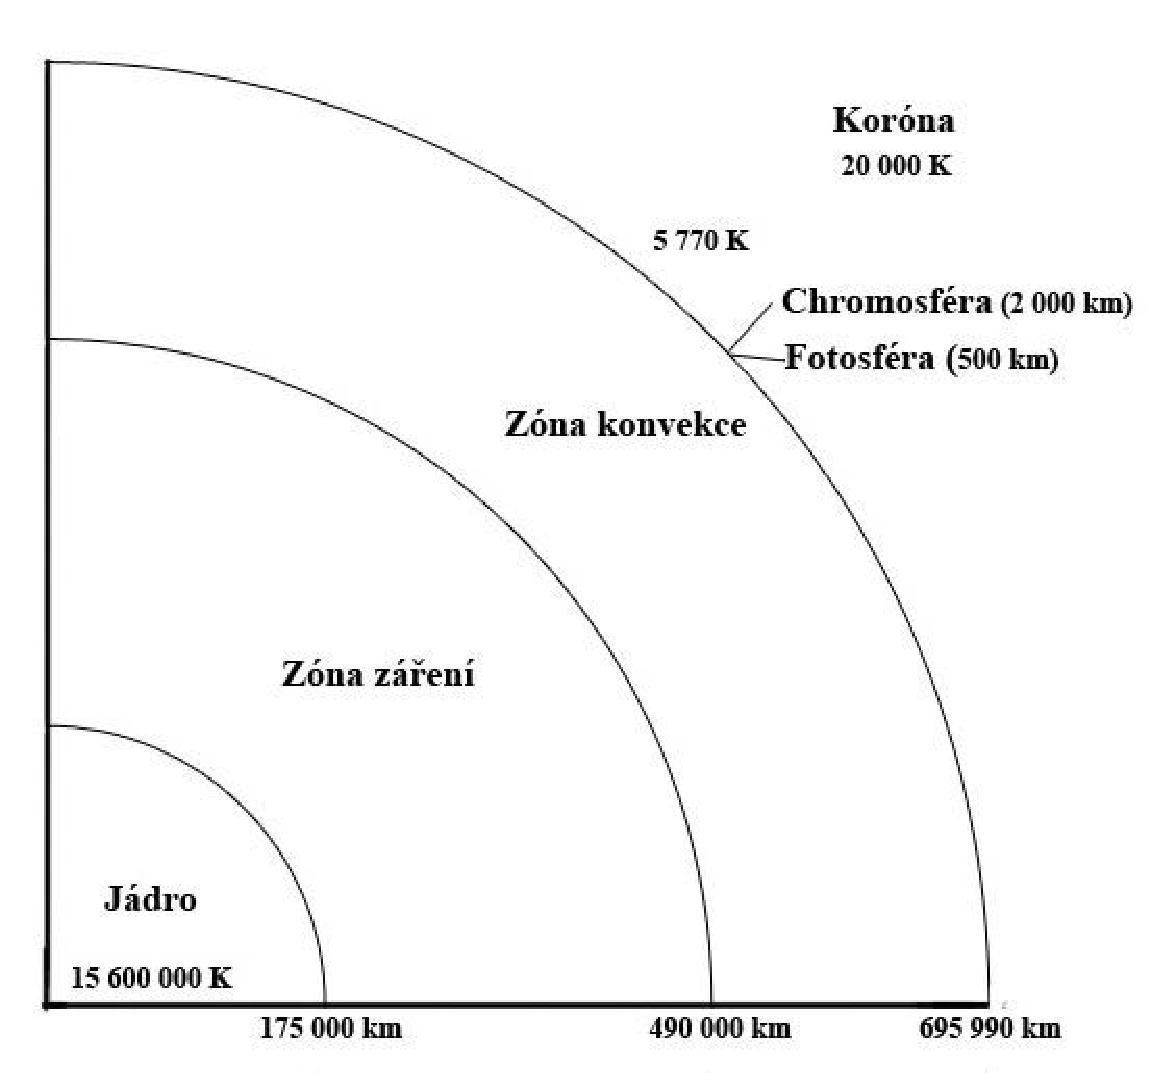
\includegraphics[scale=0.5]{../img/stavba_slunce.eps}
	\caption{Schéma jednotlivých vrstev Slunce - obrázek převzat z~\cite{astro_hvezda}}
	\label{fig:stavba}
\end{figure}
\chapter{Sluneční skvrny}

\section{Vznik slunečních skvrn}
S magnetickým polem je spojena sluneční aktivita, jako sluneční erupce, výrony koronální hmoty a sluneční skvrny. V důsledku konvektivních pohybů a diferenciální rotace není magnetické pole Slunce čistě dipólové. Jeho deformace se v celkovém součtu vyruší a z velké vzdálenosti má pole charakter dipólu, ale lokálně se projevují sluneční aktivitou. Magnetické pole v elektricky nabitém plynu doprovází magnetický tlak. V případě, že magnetická silotrubice vystoupí to fotosféry, dojde v místech, kde silotrubice vystupuje nad povrch ke snížení tlaku plynu, aby tlak plynu a magnetický tlak byl v součtu stejný, jako tlak v okolí. Oblasti s nízkým tlakem se začnou ochlazovat a v důsledku toho vznikají místa s nižší teplotou (\unit[3000-4000]{K} oproti \unit[5000-6000]{K} ve zbytku fotosféry).

Místa, kde silotrubice vystupuje do fotosféry jsou tedy chladnější a mají mnohonásobně (cca 4-5krát) menší zářivý výkon než okolí a pozorujeme je jako tmavá. V souladu s charakterem jejich původu pozorujeme sluneční skvrny ve většině případů v páru, jelikož silotrubice musí fotosféru protnout ve dvou místech. Typické rozměry slunečních skvrn se pohybují mezi $\unit[3500-60000]{km}$.

Přesný mechanismus a příčiny pro výstup silotrubice do fotosféry ovšem stále nejsou zcela objasněny.


\section{Struktura slunečních skvrn}

\subsection{Wilsonova deprese}
Pro sluneční skvrny je optické hloubky $\tau=1$ dosaženo ve větší hloubce, než v klidném Slunci (zhruba o $\unit[0.5-2]{Mm}$ hlouběji). Znamená to tedy, že fotony mající původ ve slunčení skvrně, které opustí Slunce jsou produkovány v průměrně větší hloubce, než fotony, které vidíme ze zbytku fotosféry. Tento jev se nazývá Wilsonova deprese.

Důvodem je nížší teplota a tlak plynu, než je v okolí, což má za následek snížení opacity, která s optickou hloubkou přímo souvisí.

\subsection{Jemná struktura}
Nejvýraznějšími částmi sluneční skvrny jsou \textit{umbrální jádro} a \textit{penumbra}. Umbra je jádro sluneční skvrny. Je její nejchladnější a nejtmavší částí. Umbrální jádro obklopuje penumbra, která se skládá z protáhlých, převážně radiálně orientovaných struktur. Ty jsou důsledkem odklonu magnetického pole od kolmice v okolí umbrálního jádra. Teplota penumbry je již výrazně vyšší, než teplota umbrálního jádra; dosahuje hodnot pouze zhruba o $\unit[250-400]{K}$ nižších než je teplota okolí.

V umbrálním jádře jsou pozorovány světlé body, zvané \textit{umbrální body}. Jsou projevem konvekce uvnitř sluneční skvrny a dokazují, že zde stále dochází ke konvektivnímu přenosu energie. Světlé struktury, které z vnějšku zasahují do jádra, či od sebe 2 jádra oddělují se nazývají \textit{světelné mosty}. Jsou projevem silné konvekce a vznikají při zániku slunečních skvrn z umbrálních bodů. Struktura sluneční skvrny je znázorněna na obr. \ref{fig:skvrna}

\begin{figure}[h!]
	\centering
	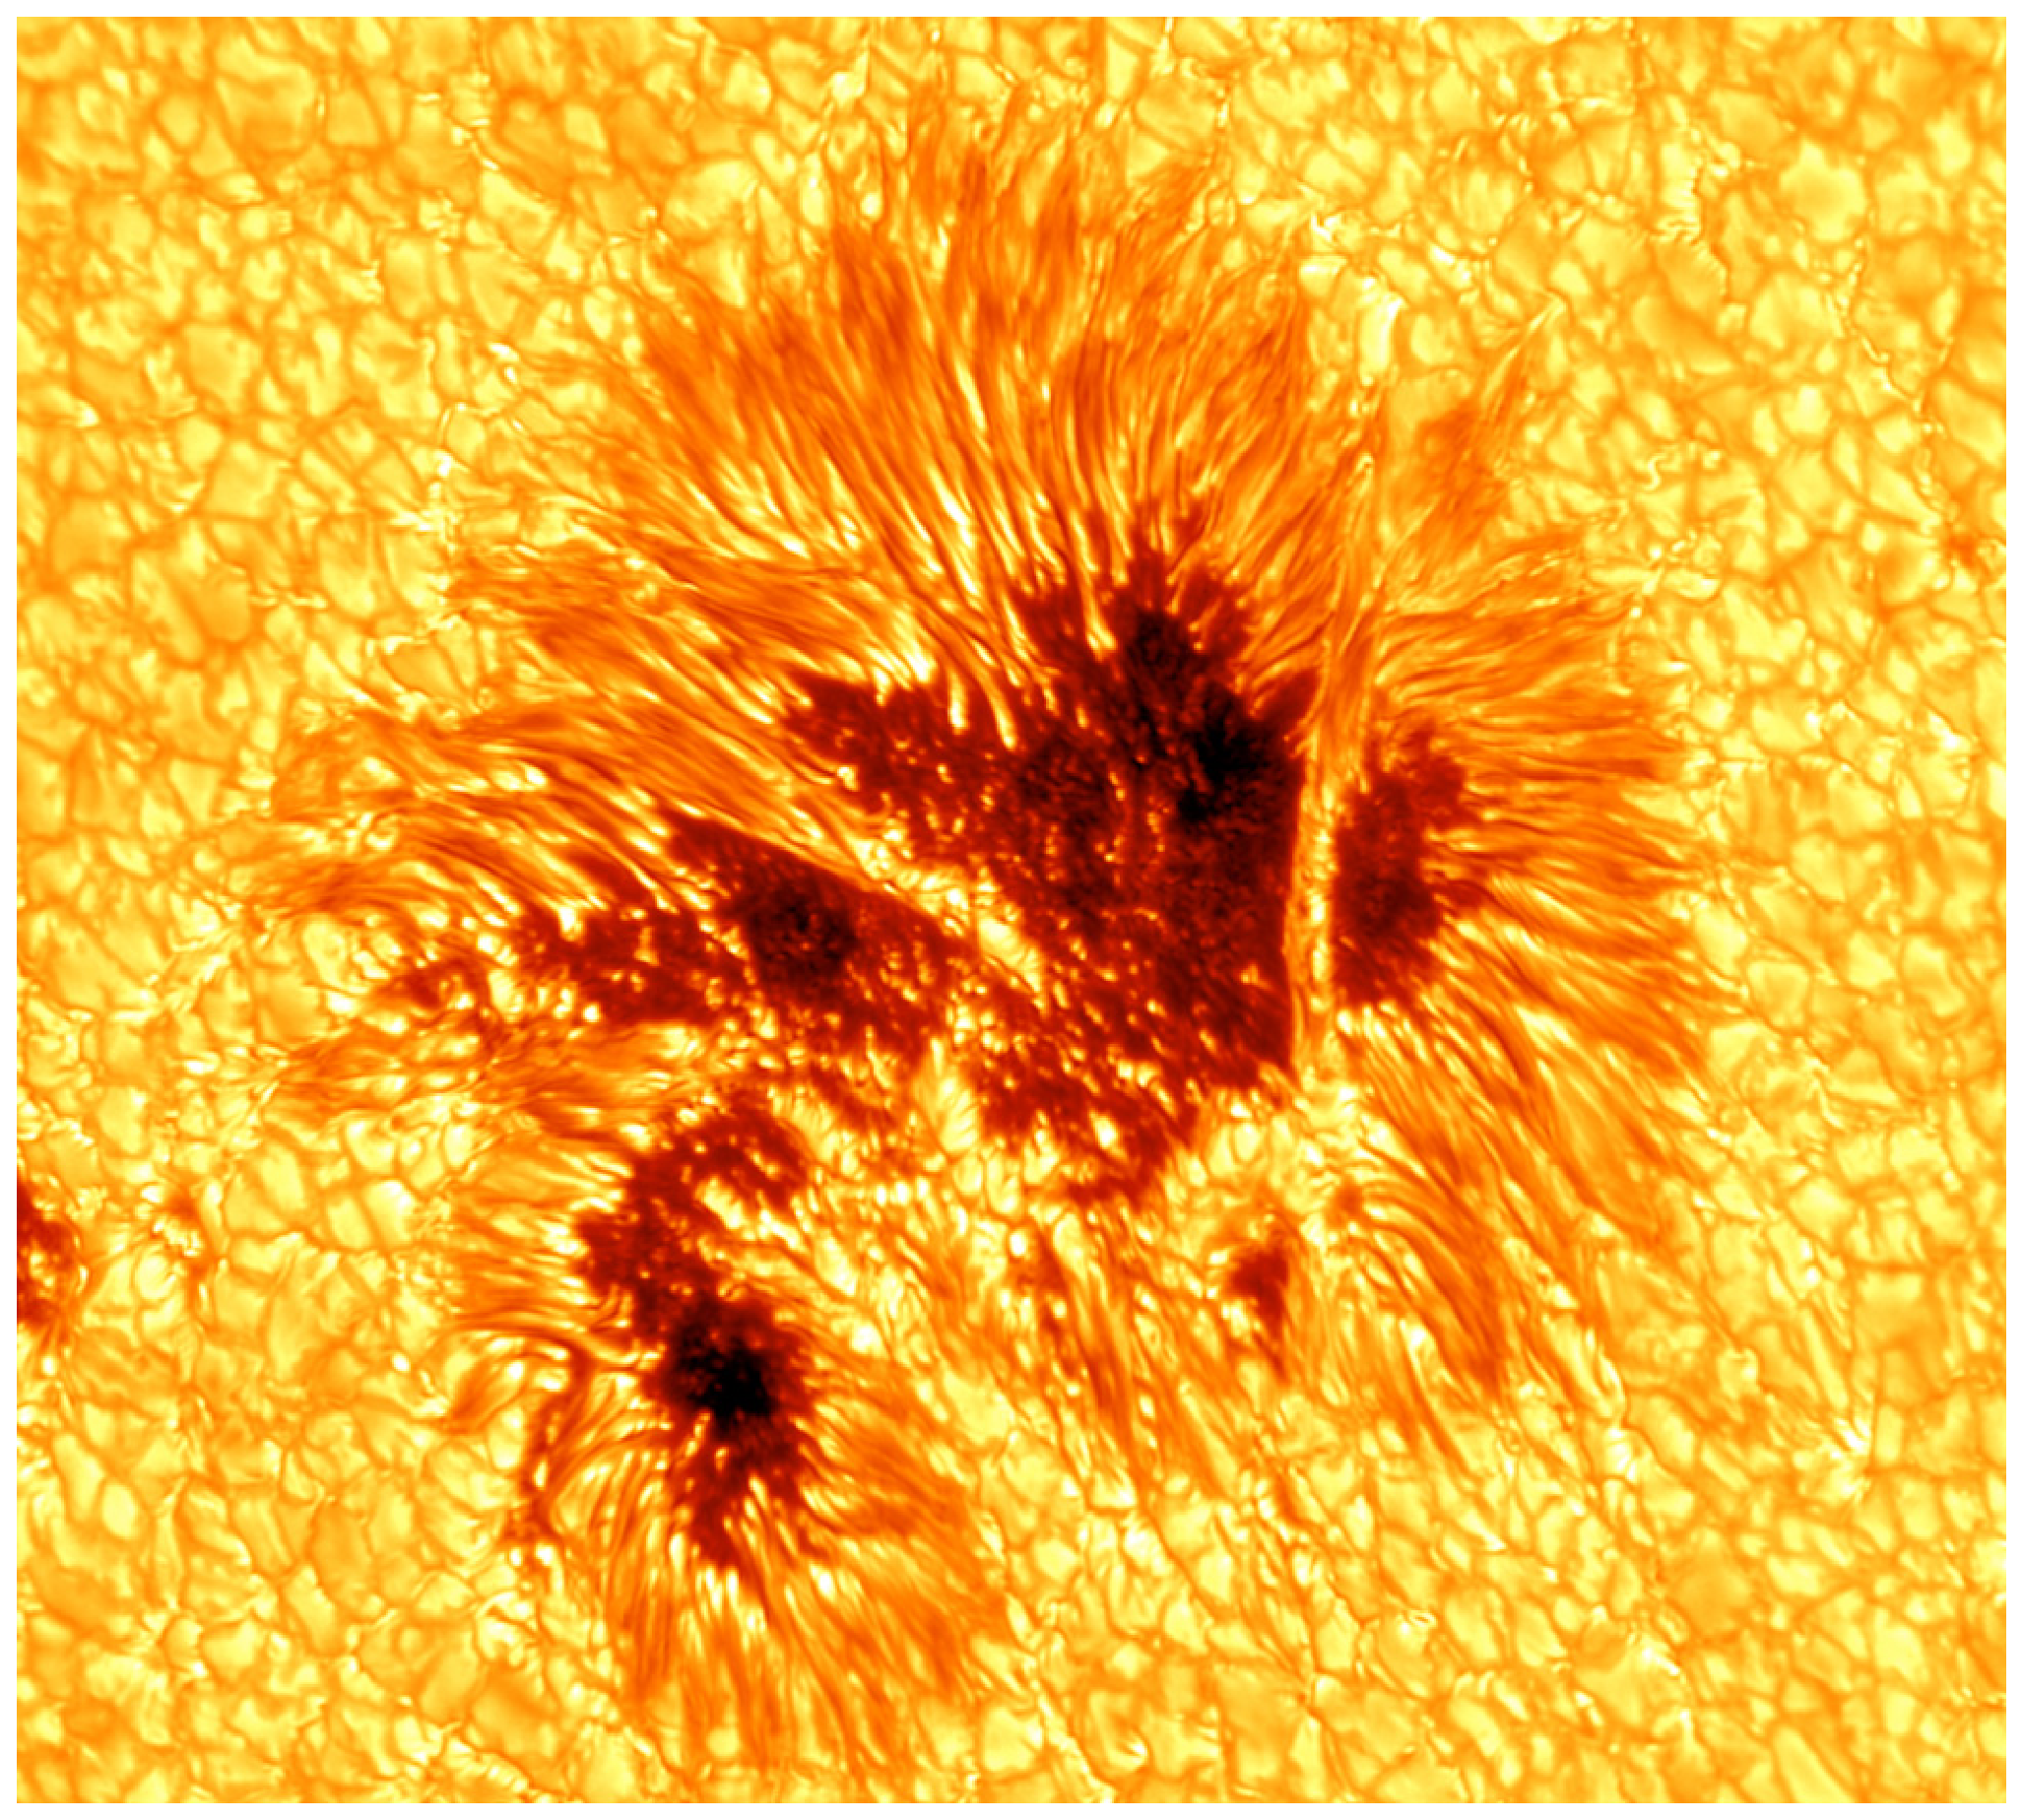
\includegraphics[scale=0.2]{../img/sunspot_structure.eps}
	\caption{zdroj: \url{http://www.extremetech.com/extreme/163460-marvel-at-the-most-detailed-photos-of-the-sun-ever-taken}}
	\label{fig:stavba}
\end{figure}


\section{Teoretické modely slunečních skvrn}
Všechny modely slunečních skvrn předpokládají, že skvrna je tvořena jednou osově symetrickou silotrubicí a ve většině modelů je soustava v magnetohydrostatické rovnováze, která je předepsána rovnováhou mezi silami uvnitř a vně silotrubice a Maxwellovou rovnicí:
\begin{align}
	\frac{1}{\mu_0}(\nabla\times\vect{B})\times\vect{B} &= \nabla p-\rho\vect{g} \label{eq:mh_equilib} \\
	\nabla\cdot\vect{B} &= 0
\end{align}
Předpoklad, že soustava je v každém okamžiku v hydrostatické rovnováze je většinou oprávněná, neboť vývoj slunečních skvrn probíhá v mnohem delších časových škálách, než je doba, po jakou se šíří vzruchy napříč silotrubicí.

\subsection{Self-similar modely}
Self-similar řešení jsou založena na předpokladu, že magnetické pole není zakroucené (tedy $B_\theta(r,z)=0$) a radiální závislost $\vect{B}$ je v každé hloubce stejná až na škálovací faktor, který zajišťuje konstantní magnetický tok při rozšiřování, nebo zužování silotrubice. Předpokládá se tedy následující:
\begin{equation}
	B_z(r,z)=f(\zeta)B_0(z),
	\label{eq:Bz}
\end{equation}
kde $B_0(z)$ je intenzita magnetického pole na ose symetrie, $\zeta=r\sqrt{B_0(z)}$ a $f(\zeta)$ je funkce určující tvar závislosti. Z Maxwellovy rovnice pro divergenci magnetického pole lze poté odvodit:
\begin{equation}
	B_r(r,z)=-rf(\zeta)\frac{\D B_0(z)}{\D z}
	\label{eq:Br}
\end{equation}
Pro zachování konstantního magnetického toku $\Phi$ silotrubicí je na funkci $f(\zeta)$ kladena podmínka
\begin{equation}
	2\pi\int\limits_0^{+\infty}f(\zeta)\zeta\,\D\zeta=\Phi.
\end{equation}
Je zvykem volit jako $f(\zeta)=\exp(-\zeta^2)$, která tuto podmínku splňuje.

Problém self-similar modelů může být, že jsou na magnetické pole kladeny příliš silné předpoklady. V modelech není skvrna vidět jako umbrální jádro obklopené penumbrou. Důkladnější modely také ukazují, že podmínka soběpodobnosti ve skutečnosti nejspíše není splněna.
\chapter{Dynamická diskonexe}

Pozorování bipolárních slunečních skvrn nasvědčuje, že pár dní po jejich vynoření se silotrubice, která je tvoří, odpojí od magnetického jádra Slunce. Důvody jsou následující:
\begin{itemize}
	\item Velikost aktivních oblastí, kde skvrny vznikají, je mnohem rozsáhlejší, než je vzájemná vzdálenost dvou bipolárních skvrn. Kdyby tedy silotrubice byla dále napojena na magnetické jádro a vynořovala by se, očekávali bychom, že vzájemná vzdálenost skvrn bude odpovídat rozměrům dané aktivní oblasti. Vzdálenost skvrn ovšem v porovnání s velikostí aktivní oblasti zůstane nepatrná.
	\item Skvrny by se měly pohybovat směrem k pólům (tento jev nepozorujeme) \textbf{není mi jasné proč}
	\item Při vynořování na magnetickou silotrubici působí Coriolisova síla, která způsobí natočení spojnice skrvn vůči východo-západnímu směru. Poté, co vynořování skončí, Coriolisova síla přestává působit a očekáváme, že naklonění spojnice bude relaxovat zpět do jeho původní polohy; ani tento jev ovšem nepozorujeme.
\end{itemize}

Mechanismus navržený ve článku \cite{dd} se snaží vysvětlit z jakého důvodu a jak k odpojení od magnetického jádra.

Po vynoření sluneční skvrny se její povrch začne ochlazovat, což je doprovázeno tokem plynu směrem ke středu Slunce. Tím dojde k poklesu tlaku v povrchové vrstvě skvrny a zesílení magnetického pole v této oblasti. V hloubce mezi $\unit[2-10]{Mm}$ dojde vlivem toku plynu směřujícího do hloubky k nárůstu tlaku a po několika dnech tento tlak v určitém místě vyrovná tlak v okolí silotrubice a dojde k rozpojení silotrubice.

\section{Model dynamické diskonexe a model konvekce}

\subsection{Model konvekce}
Pozorování (viz. umbrální tečky) nasvědčuje tomu, že ve slunečních skvrnách nedochází pouze k radiativnímu přenosu energie, ale také ke konvektivnímu přenosu. Z rovnic hvězdného nitra vyplývá pro celkový tok a tok energie přenášený radiací
\begin{align}
	F_{rad}+F_{conv} &= \frac{4acG}{3}\frac{mT^4}{\kappa P r^2}\nabla_{rad} \label{eq:celk_tok}\\
	F_{rad} &= \frac{4acG}{3}\frac{mT^4}{\kappa P r^2}\nabla \label{eq:frad}
\end{align}
kde $\nabla_{rad}=\left(\frac{\D\ln T}{\D\ln p}\right)_e$ je logaritmický teplotní gradient potřebný pro to, aby energie byla přenášena pouze zářením, $\nabla$ je skutečný logaritmický teplotní gradient.

Skutečný teplotní gradient a tedy i vztah pro tok energie přenášené konvekcí záleží na použitém modelu konvekce. Pro astrofyzikální aplikace se velmi často používá model směšovacích délek (mixing length model).

Tento zjednodušující model předpokládá, že energie je přenášena elementem hmoty, který se po určitou dobu chová jako uzavřený systém o konstantním počtu částic a po určité uražené vzdálenosti (směšovací délce $l_m$) difunduje do okolí. Definujme pro veličinu $X$ operátor:
\begin{equation}
	DX = \left(\left(\frac{\D X}{\D z}\right)_e-\frac{\D X}{\D z}\right)\Delta r,
\end{equation}
kde $\left(\frac{\D X}{\D z}\right)_e$ je změna veličiny uvnitř elementu způsobená zvětšováním objemu pro zachování stejného tlaku, jako je v okolí (tedy $Dp=0$) a radiačními energetickými ztrátami. Potom bude po uražení vzdálenosti $\Delta r$ bude rozdíl mezi teplotou elementu a teplotou okolí
\begin{equation}
	D T = \left(\nabla_e-\nabla\right)\frac{T\Delta r}{H_p}, \label{eq:nne}
\end{equation}
kde $\nabla$ a $\nabla_e$ jsou logaritmické gradienty teploty vztažené k logaritmu tlaku, $H_p=\frac{\D z}{\D\ln p}$. Elementem o hustotě $\rho$, měrné tepelné kapacitě $c_p$ pohybujícím se rychlostí $v$ je čistě konvekcí přenesena energie $E_{conv}=\rho c_p D T$ a konvektivní energetický tok je tedy
\begin{equation}
	F_{conv} = \rho c_p v D T.
\end{equation}
Předpokládejme, že součin $vDT$ bude nabývat své střední hodnoty poté, co element urazí vzdálenost $\frac{l}{2}$. Element bude v důsledku vztlaku urychlován silou, jejíž hustota je
\begin{equation}
	k_r=-g \frac{D\rho}{\rho}=-g\pder[\ln\rho]{\ln T}\frac{DT}{T}=-g\delta\frac{DT}{T},
\end{equation}
kde
\begin{equation}
	\delta=\pder[\ln\rho]{\ln T}.
\end{equation}
Práce vztažená na jednotku hmotnosti po uražení vzdálenosti $l_m/2$ je tedy
\begin{equation}
	W = k_r\frac{l_m}{2}=\frac{1}{8}g\delta\frac{l_m^2}{H_p}(\nabla-\nabla_e).
\end{equation}
Za předpokladu, že práce je z poloviny vynaložena na odpor prostředí a z poloviny na kinetickou energii, můžeme střední rychlost $v$ určit ze vztahu
\begin{equation}
	\frac{1}{2}v^2=\frac{1}{2}W
\end{equation}
a tedy
\begin{equation}
	F_{conv} = \rho c_p T\sqrt{g\delta}\frac{l^2_m}{4\sqrt{2}}H_p^{-3/2}(\nabla-\nabla _e)^{3/2}. \label{eq:fconv1}
\end{equation}
Nebýt radiativního ochlazování elementu, platilo by $\nabla_e=\nabla_{ad}$. $\nabla_{ad}$ je tzv. adiabatický teplotní gradient, který lze lokálně spočítat pomocí vztahu
\begin{equation}
	\nabla_{ad}=\frac{\delta P}{c_P\rho T}
\end{equation}
Hustotu toku energie, kterou element vyzařuje lze v difúzní aproximaci vyjádřit jako
\begin{equation}
	f = \frac{-4ac}{3}\frac{T^3}{\kappa\rho}\frac{\D T}{\D n}.
\end{equation}
Normálový teplotní gradient $\frac{\D T}{\D n}$ můžeme pro kouli o průměru $d$ aproximovat jako $\frac{DT}{d/2}$ a tedy celkový zářivý výkon $\lambda$ takové koule je
\begin{align}
	\lambda &= Sf\\
			&= \frac{8acT^3}{3\kappa\rho}DT\frac{S}{d}.
\end{align}
Odtud již můžeme určit odchylku od změny při adiabatickém ději, jelikož $\frac{\D T}{\D r} = \frac{\D T}{\D Q}\frac{\D Q}{\D t}\frac{\D t}{\D r}$. Proto
\begin{align}
	\left(\frac{\D T}{\D r}\right)_e-\left(\frac{\D T}{\D r}\right)_{ad} &= -\frac{\lambda}{\rho V c_p v}\\
	\nabla _e-\nabla _{ad} &= \frac{8ac}{3\kappa}DT\frac{6}{d^2}.
\end{align}
Vydělením rovnicí (\ref{eq:nne}):
\begin{equation}
	\frac{\nabla _e-\nabla _{ad}}{\nabla-\nabla _e} = \frac{8acT^3}{\kappa\rho^2vc_p}\left(\frac{l_m}{d^2}\right).
\end{equation}
Element ovšem není dokonalá koule, proto se člen $\frac{8l_m}{d^2}$ nahrazuje $\frac{6}{l_m}$. Dále lze kombinací rovnic (\ref{eq:celk_tok}) a (\ref{eq:fconv1}) za použití $g=\frac{Gm}{r^2}$ vyjádřit
\begin{equation}
	F_{conv} = \rho c_p T\sqrt{g\delta}\frac{l^2_m}{4\sqrt{2}}H_p^{-3/2}\frac{8U}{9}(\nabla_{rad}-\nabla). \label{eq:fconv}
\end{equation}
V případě, že je známa závislost teploty na tlaku, lze z tohoto vzorce v každém bodě spočítat veličinu $F_{conv}$.

\subsection{Magnetohydrostatická rovnováha}
Dosazením magnetického pole v soběpodobném tvaru podle rovnic (\ref{eq:Bz}) a (\ref{eq:Br}) do rovnice pro magnetohydrostatickou rovnováhu (\ref{eq:mh_equilib}) získáme následující dvě rovnice pro magnetohydrostatickou rovnováhu:
\begin{align}
	0 &= -\pder[p]{r}+\frac{B_z}{\mu_0}\left(\pder[B_r]{z}-\pder[B_z]{r}\right)\\
	0 &= -\pder[p]{z}-\frac{B_r}{\mu_0}\left(\pder[B_r]{z}-\pder[B_z]{r}\right)-\rho g
\end{align}
První z těchto rovnic po integrování podle $r$ od $0$ do $\infty$ (pro konstantní $z$) přechází v rovnici
\begin{equation}
	\frac{\Phi}{2\pi}y\frac{\D^2y}{\D z^2}=y^4-2\mu_0(p_e-p_i), \label{eq:magstat}
\end{equation}
kde $y=\sqrt{B_0(z)}$, $\Phi$ je magnetický tok silotrubicí (nezávislý na hloubce), $p_e(z)=p(\infty,z)$ je vnější tlak a $p_i(z)=p(0,z)$ je tlak uvnitř silotrubice, který j dán podmínkou pro hydrostatickou rovnováhu:
\begin{equation}
	\frac{\D p_i}{\D z}=\rho_i g \label{eq:hydrostat}
\end{equation}

\subsection{Časový vývoj}
Jde o kvazistacionární model, předpokládá se tedy, že v každém okamžiku je soustava v magnetohydrostatické rovnováze, která je určena rovnicemi (\ref{eq:magstat}) a (\ref{eq:hydrostat}). V důsledku přenosu energie se ovšem v průběhu mění teplota a v důsledku toku plynu směrem od středu Slunce na povrch se bude měnit také tlak.

Pro změnu teploty $T_i$ v důsledku přenosu energie platí
\begin{equation}
	\pder[T_i]{t}=-\frac{1}{\rho_i c_p} \pder[]{z}(F_{rad}+F_{conv}),
\end{equation}
kde $F_{rad}$ a $F_{conv}$ jsou dány vztahy (\ref{eq:frad}) a (\ref{eq:fconv}).

V případě tenké silotrubice lze celkovou hmotu v silotrubici odhadnout vztahem
\begin{equation}
	m = \Phi\int\limits_0^{z_0}\frac{\rho_i}{B}\,\D z.
\end{equation}
Pokud na hranici $z_0$ vtéká hmota rychlostí $v_0$, lze tedy tuto změnu vyjádřit jako
\begin{equation}
	\Delta m=\Phi\frac{\rho_i(z_0)}{B(z_0)}v_0\Delta t.
\end{equation}
Změna tlaku v hloubce $z_0$ za časový úsek $\Delta t$ tedy musí být taková, aby bylo splněno
\begin{equation}
	m[p_i(z_0)+\Delta p_i(z_0)]=m[p_i(z_0)]+\Phi\frac{\rho_i(z_0)}{B(z_0)}v_0\Delta t
\end{equation}
\chapter{Simulace dynamické diskonexe}

\section{Model klidného Slunce}
Pro umožnění spočtení magnetického pole podle rovnice (\ref{eq:magstat}) je potřeba znát tlak plynu jako funkci hloubky v klidném Slunci $p_e(z)$. Za tímto účelem lze použít některý dostupných modelů. Výpočet byl ovšem v rámci práce pro přípovrchvé vrstvy proveden pro ověření správnosti použitého modelu konvekce.

\subsection{Rovnice přenosu energie}
V difúzní aproximaci lze logaritmický teplotní zářivý gradient $\nabla_{rad}$ vypočítat podle vztahu
\begin{equation}
	\frac{3\kappa P L_R}{16\pi a c G M_R T^4},
\end{equation}
kde $L_R$ je celkový zářivý výkon Slunce ve vzdálenosti $R$ od jeho středu, $M_R$ je hmotnost části Slunce obalené slupkou o poloměru $R$. V přípovrchových vrstvách, kterými se v práci zabýváme, dochází již pouze k naprosto zanedbatelnému počtu jaderných reakcí, při kterých by byla produkována energie a které by ovlivnily celkový zářivý výkon. Proto byla pro výpočet tato hodnota nahrazena hodnotou $L^*$, tedy zářivým výkonem celého Slunce. Tento gradient určuje, jak se mění teplota v závislosti na tlaku, pokud uvažujeme pouze zářivý přenos energie.

Označme logaritmický teplotní gradient získaný z modelu konvekce jako $\nabla_{conv}$. Jelikož bude vždy automaticky zvolen efektivnější způsob přenosu energie, můžeme pro skutečný teplotní gradient $\nabla$ psát
\begin{equation}
	\nabla = \min(\nabla_{ad},\nabla_{conv}).
\end{equation}

% Ukázka použití některých konstrukcí LateXu (odkomentujte, chcete-li)
% %%% Ukázka použití některých konstrukcí LaTeXu

\subsection{Ukázka \LaTeX{}u}
\label{ssec:ukazka}

V~této krátké části ukážeme použití několika základních konstrukcí \LaTeX{}u,
které by se vám mohly při psaní práce hodit.

Třeba odrážky:

\begin{itemize}
\item Logo Matfyzu vidíme na obrázku~\ref{fig:mff}.
\item Tato subsekce má číslo~\ref{ssec:ukazka}.
\item Odkaz na literaturu~\cite{lamport94}.
\end{itemize}

Druhy pomlček:
červeno-černý (krátká),
strana 16--22 (střední),
$45-44$ (minus),
a~toto je --- jak se asi dalo čekat --- vložená věta ohraničená dlouhými pomlčkami.
(Všimněte si, že jsme za \verb|a| napsali vlnovku místo mezery: to aby se
tam nemohl rozdělit řádek.)

% Makro na české uvozovky (novější verze LaTeXu ho už mají zabudované)
\newcommand{\uv}[1]{\quotedblbase #1\textquotedblleft}
\uv{České uvozovky.}

\newtheorem{theorem}{Věta}
\newtheorem*{define}{Definice}	% Definice nečíslujeme, proto "*"

\begin{define}
{\sl Strom} je souvislý graf bez kružnic.
\end{define}

\begin{theorem}
Tato věta neplatí.
\end{theorem}

\begin{proof}
Neplatné věty nemají důkaz.
\end{proof}

\begin{figure}
	\centering
	
\includegraphics[width=30mm]{../img/logo.eps}
	\caption{Logo MFF UK}
	\label{fig:mff}
\end{figure}


\chapter*{Závěr}
\addcontentsline{toc}{chapter}{Závěr}


%%% Seznam použité literatury
%%% Seznam použité literatury je zpracován podle platných standardů. Povinnou citační
%%% normou pro bakalářskou práci je ISO 690. Jména časopisů lze uvádět zkráceně, ale jen
%%% v kodifikované podobě. Všechny použité zdroje a prameny musí být řádně citovány.

\def\bibname{Seznam použité literatury}
\begin{thebibliography}{99}
\addcontentsline{toc}{chapter}{\bibname}

%\bibitem{lamport94}
%  {\sc Lamport,} Leslie.
%  \emph{\LaTeX: A Document Preparation System}.
%  2. vydání.
%  Massachusetts: Addison Wesley, 1994.
%  ISBN 0-201-52983-1.

\end{thebibliography}


%%% Tabulky v bakalářské práci, existují-li.
\chapwithtoc{Seznam tabulek}

%%% Použité zkratky v bakalářské práci, existují-li, včetně jejich vysvětlení.
\chapwithtoc{Seznam použitých zkratek}

%%% Přílohy k bakalářské práci, existují-li (různé dodatky jako výpisy programů,
%%% diagramy apod.). Každá příloha musí být alespoň jednou odkazována z vlastního
%%% textu práce. Přílohy se číslují.
\chapwithtoc{Přílohy}

\openright
\end{document}
